\documentclass[aspectratio=169,11pt,xcolor=dvipsnames]{beamer}
\usepackage{graphicx} % For including graphics.
\usepackage{hyperref} % For links.
\usepackage{multirow}
\usepackage{minted}

\title{Computer Graphics with Clojure, LWJGL, and Fastmath}
\author{Jan Wedekind}
\date{Saturday, October 18th 2025}

\hypersetup{pdftitle          = {Computer Graphics with Clojure, LWJGL, and Fastmath},
            pdfsubject        = {rendering NASA CGI Moon Kit data using Clojure, LWJGL, and Fastmath},
            pdfauthor         = {Jan Wedekind},
            pdfkeywords       = {Clojure, LWJGL, Fastmath, rendering, NASA, Moon, graphics},
            pdfcreator        = {LaTeX with Beamer class},
            pdfproducer       = {TeX Live 2025/dev/Debian},
            bookmarksopen     = false,
            bookmarksnumbered = true,
            colorlinks        = true,
            filecolor         = cyan,
            citecolor         = green,
            linkcolor         = blue,
            urlcolor          = blue}

\usebackgroundtemplate{
\includegraphics[width=\paperwidth,height=\paperheight]{slide}}

\setbeamersize{text margin left=0.5cm,
               text margin right=0.5cm}

\usecolortheme{seahorse}



\definecolor{slidecolor}{rgb}{0.65,0.71,0.72}
\setbeamercolor{titlelike}{fg=black,bg=slidecolor!60}
\setbeamercolor{frametitle}{fg=black,bg=slidecolor!100}

\begin{document}

\begin{frame}
  \pdfbookmark[1]{Title}{title}
  \titlepage{}
\end{frame}

\begin{frame}
  \pdfbookmark[1]{About Me}{bio}
  \frametitle{About Me}
  \begin{minipage}[b]{0.79\textwidth}
    \begin{itemize}
      \item As a kid: playing with Omikron Basic, Borland Pascal
      \item Computer Science at Karlsruhe University
        \begin{itemize}
          \item compiler construction, robotics, measurement engineering
        \end{itemize}
      \item PhD on Computer Vision using Ruby at Sheffield Hallam University
      \item Computer Vision and Machine Learning in Industry
        \begin{itemize}
          \item Using C++, Ruby, Python
        \end{itemize}
      \item Hobby projects
        \begin{itemize}
          \item C++, Ruby, GNU Guile, Clojure
        \end{itemize}
    \end{itemize}
  \end{minipage}
  \begin{minipage}[b]{0.2\textwidth}
    
\includegraphics[width=\textwidth]{avatar}\\
    \begin{tiny}
      \url{https://www.wedesoft.de/}
    \end{tiny}
  \end{minipage}
\end{frame}

\begin{frame}
  \pdfbookmark[1]{Space Flight Simulator Examples}{stateoftheart}
  \frametitle{Space Flight Simulator Examples}
  \begin{minipage}[t]{0.49\textwidth}
    \begin{center}
      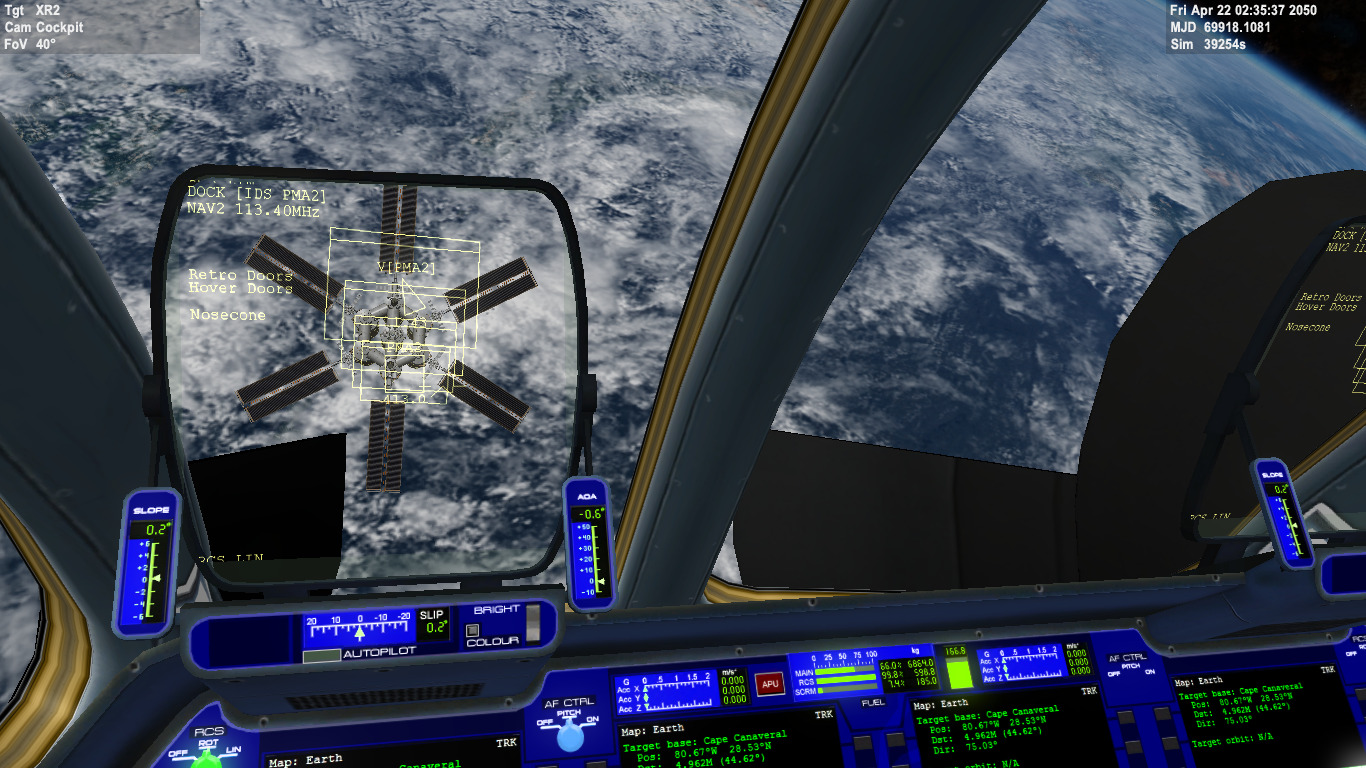
\includegraphics[width=\textwidth]{orbiter}\\
      \href{https://openorbiter.space/}{Open Orbiter Sim}\\
      former Orbiter 2016, open source since 2021, realistic, many mods
    \end{center}
  \end{minipage}
  \begin{minipage}[t]{0.49\textwidth}
    \begin{center}
      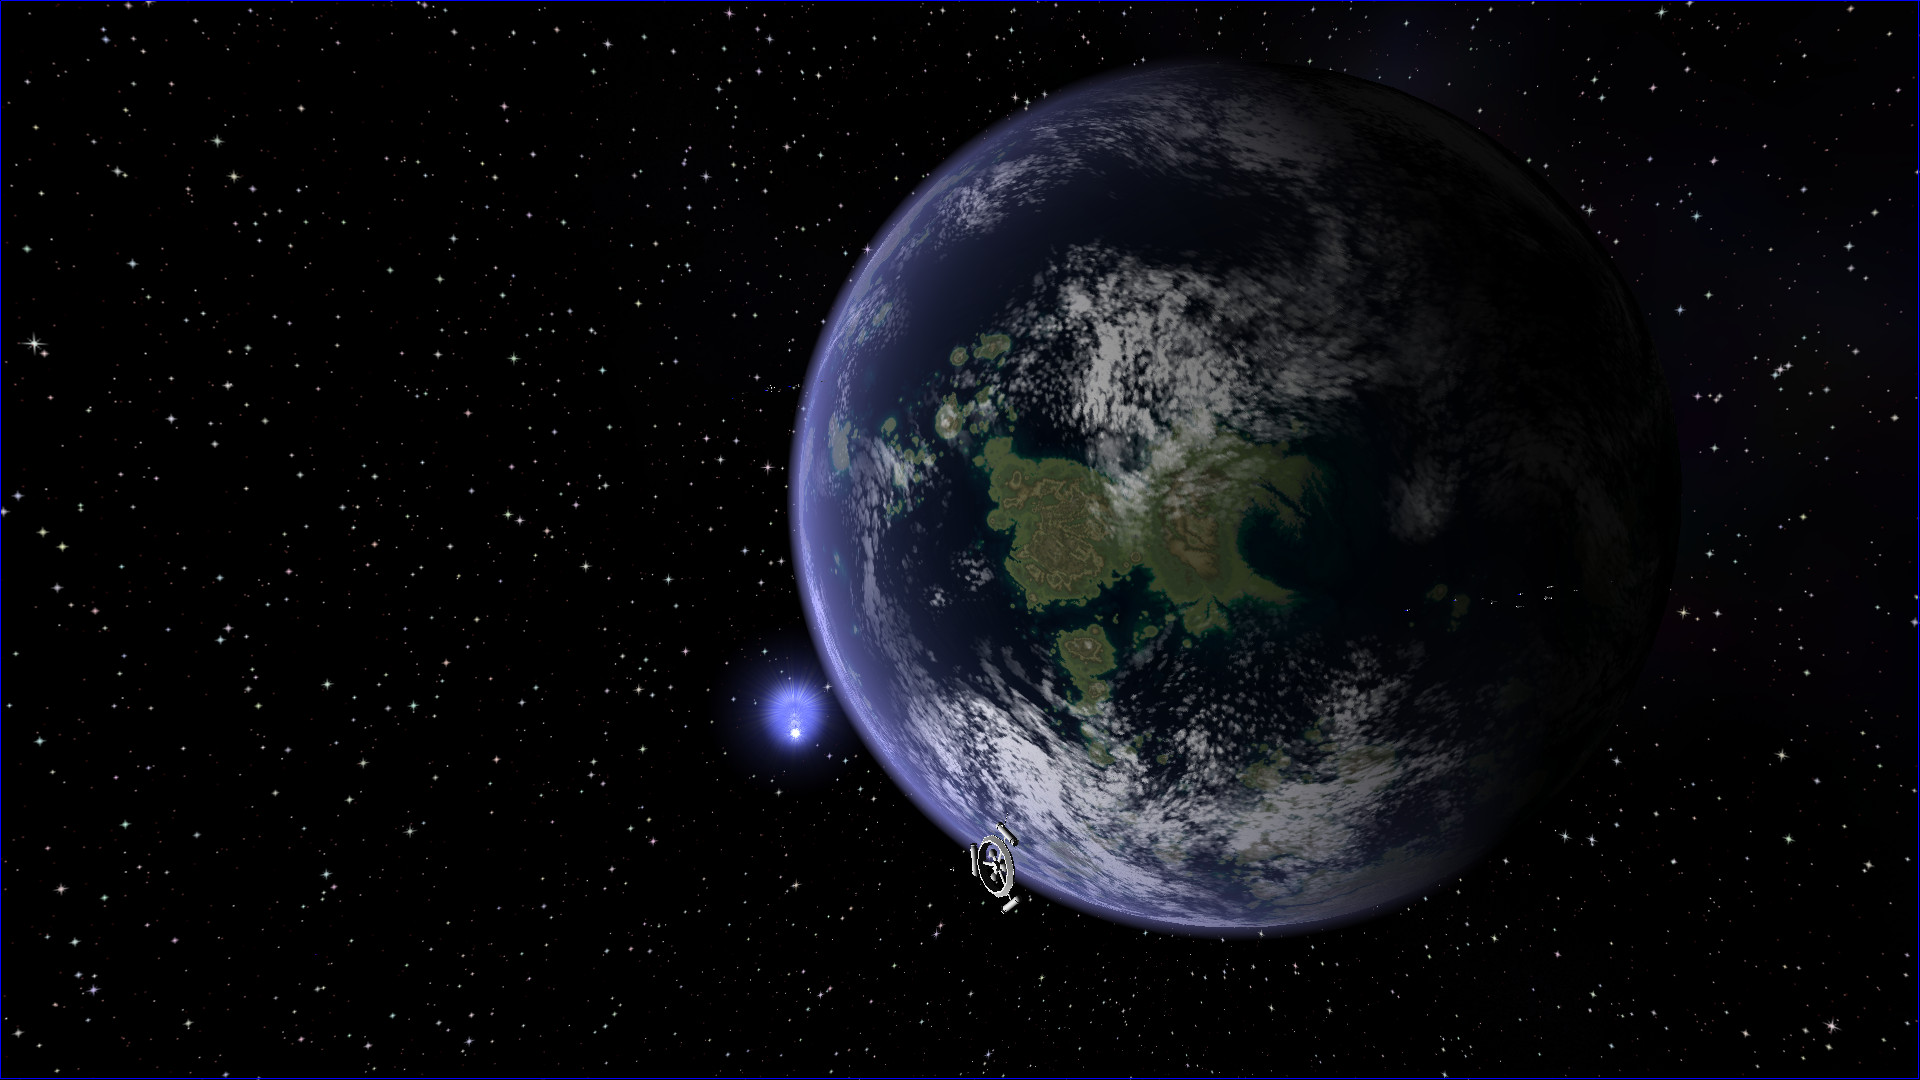
\includegraphics[width=\textwidth]{nerds}\\
      \href{https://smcameron.github.io/space-nerds-in-space/}{Space Nerds in Space}\\
      multiplayer star ship bridge sim, open source
    \end{center}
  \end{minipage}
\end{frame}

\begin{frame}
  \frametitle{Space Flight Simulator Examples}
  \begin{minipage}[t]{0.49\textwidth}
    \begin{center}
      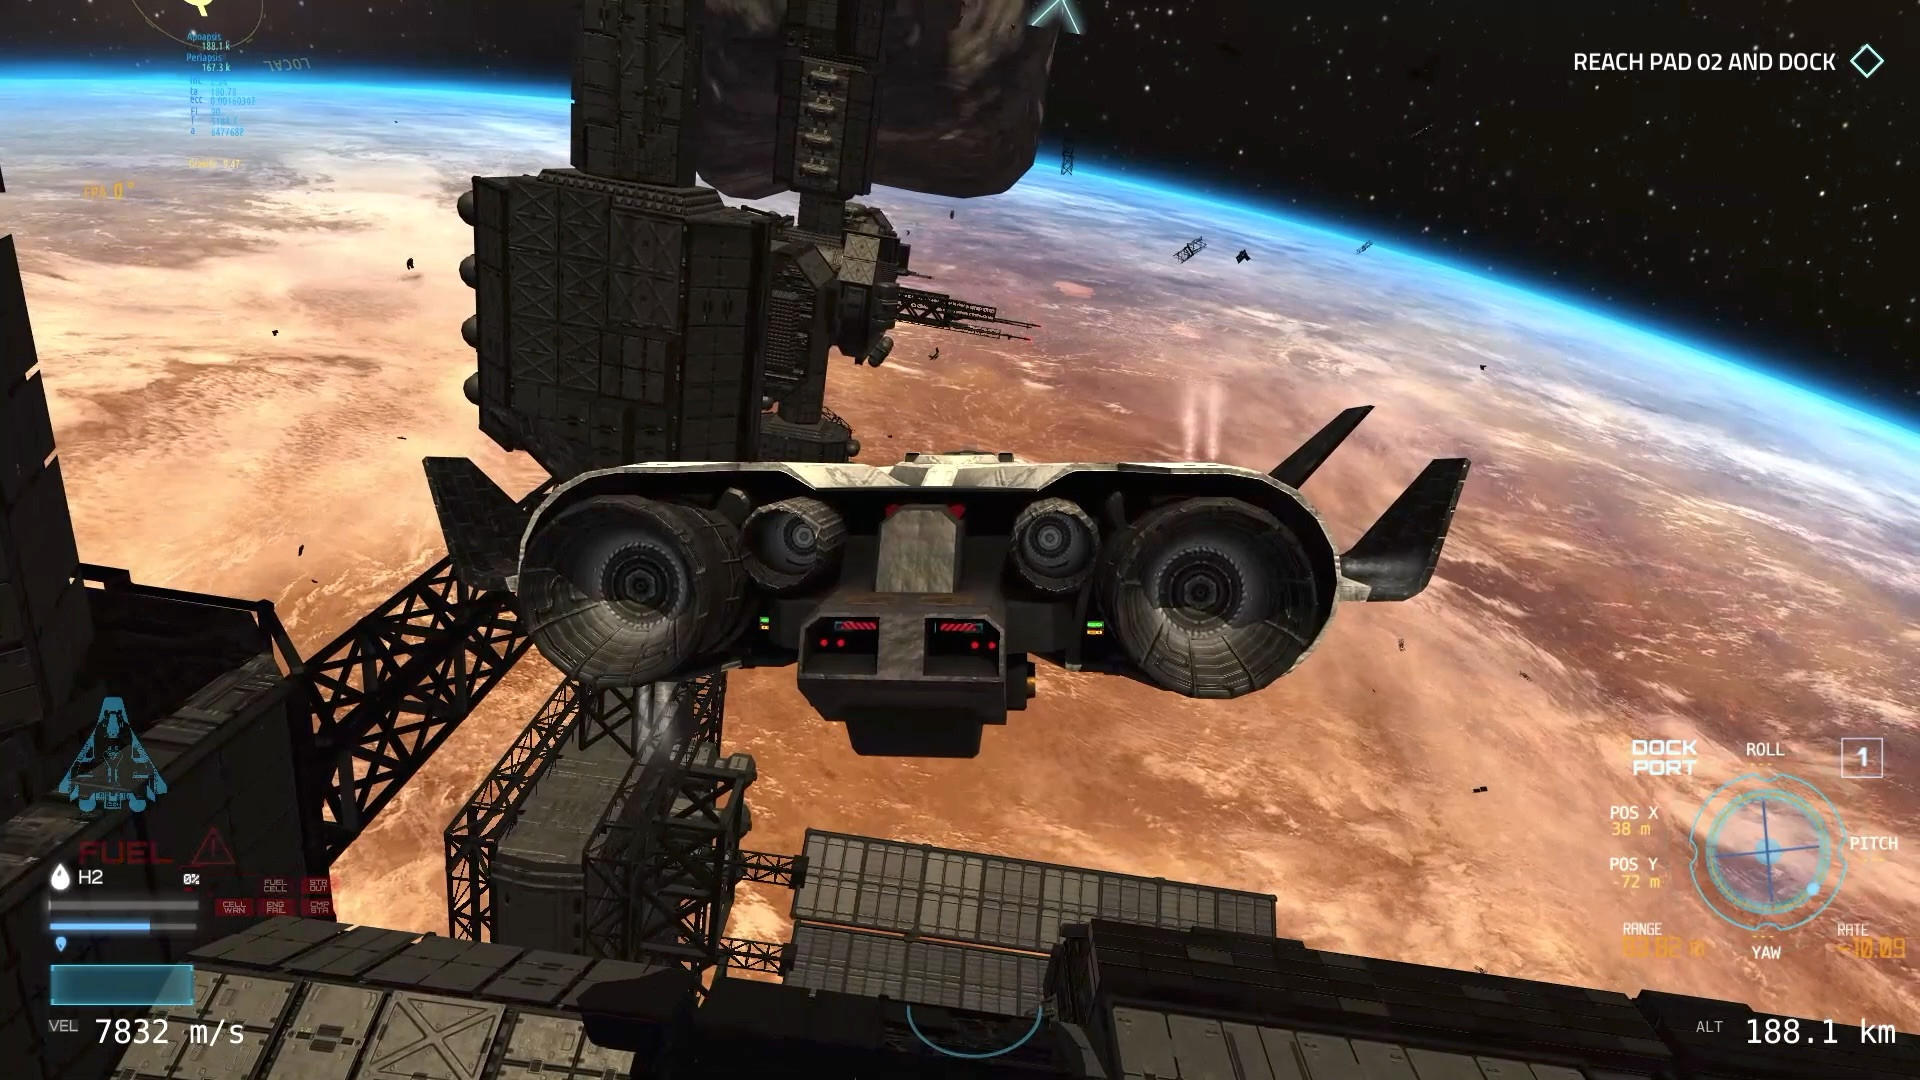
\includegraphics[width=\textwidth]{flight-of-nova}\\
      \href{https://flight-of-nova.com/}{Flight of Nova}\\
      proprietary, realistic, early access
    \end{center}
  \end{minipage}
  \begin{minipage}[t]{0.49\textwidth}
    \begin{center}
      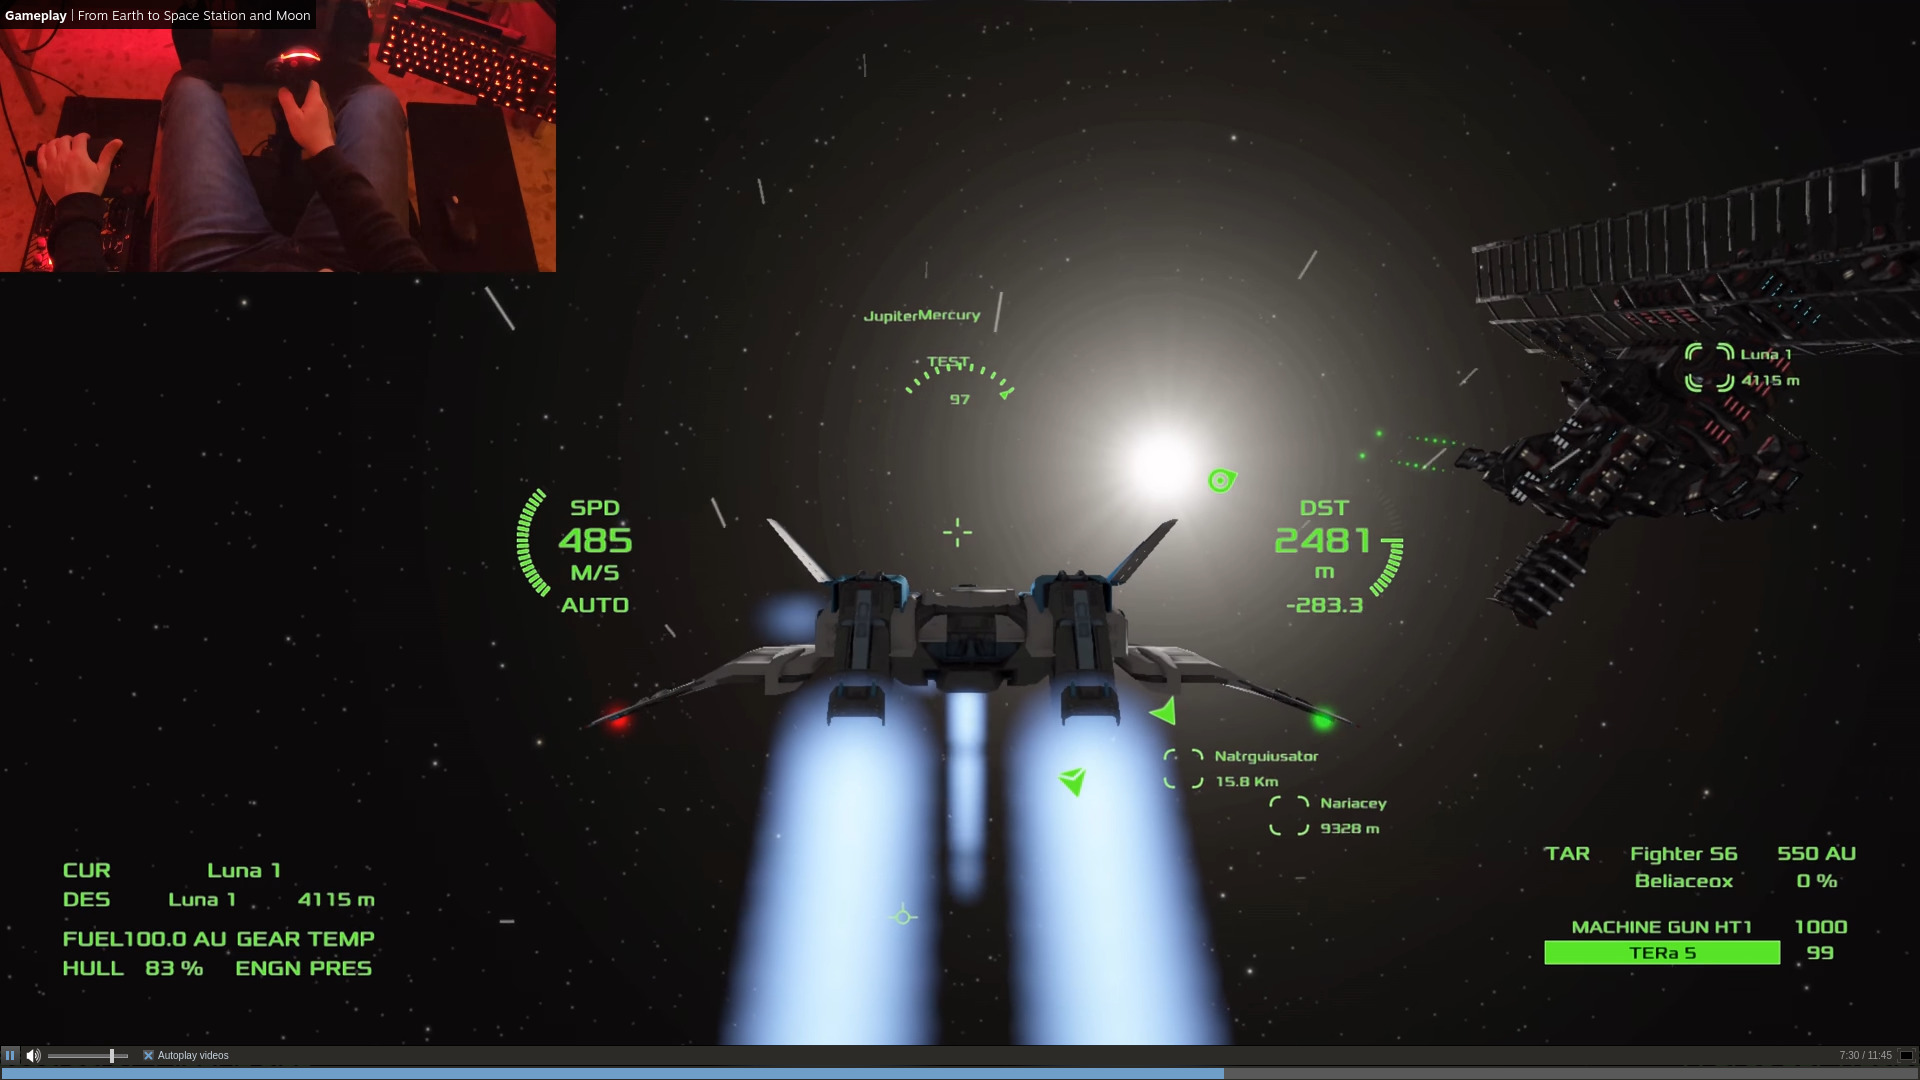
\includegraphics[width=\textwidth]{univoyager}\\
      \href{https://www.univoyager.com/}{Univoyager}\\
      proprietary, real terrain with procedural detail, to be released
    \end{center}
  \end{minipage}
\end{frame}

\begin{frame}
  \frametitle{Space Flight Simulator Examples}
  \begin{minipage}[t]{0.49\textwidth}
    \begin{center}
      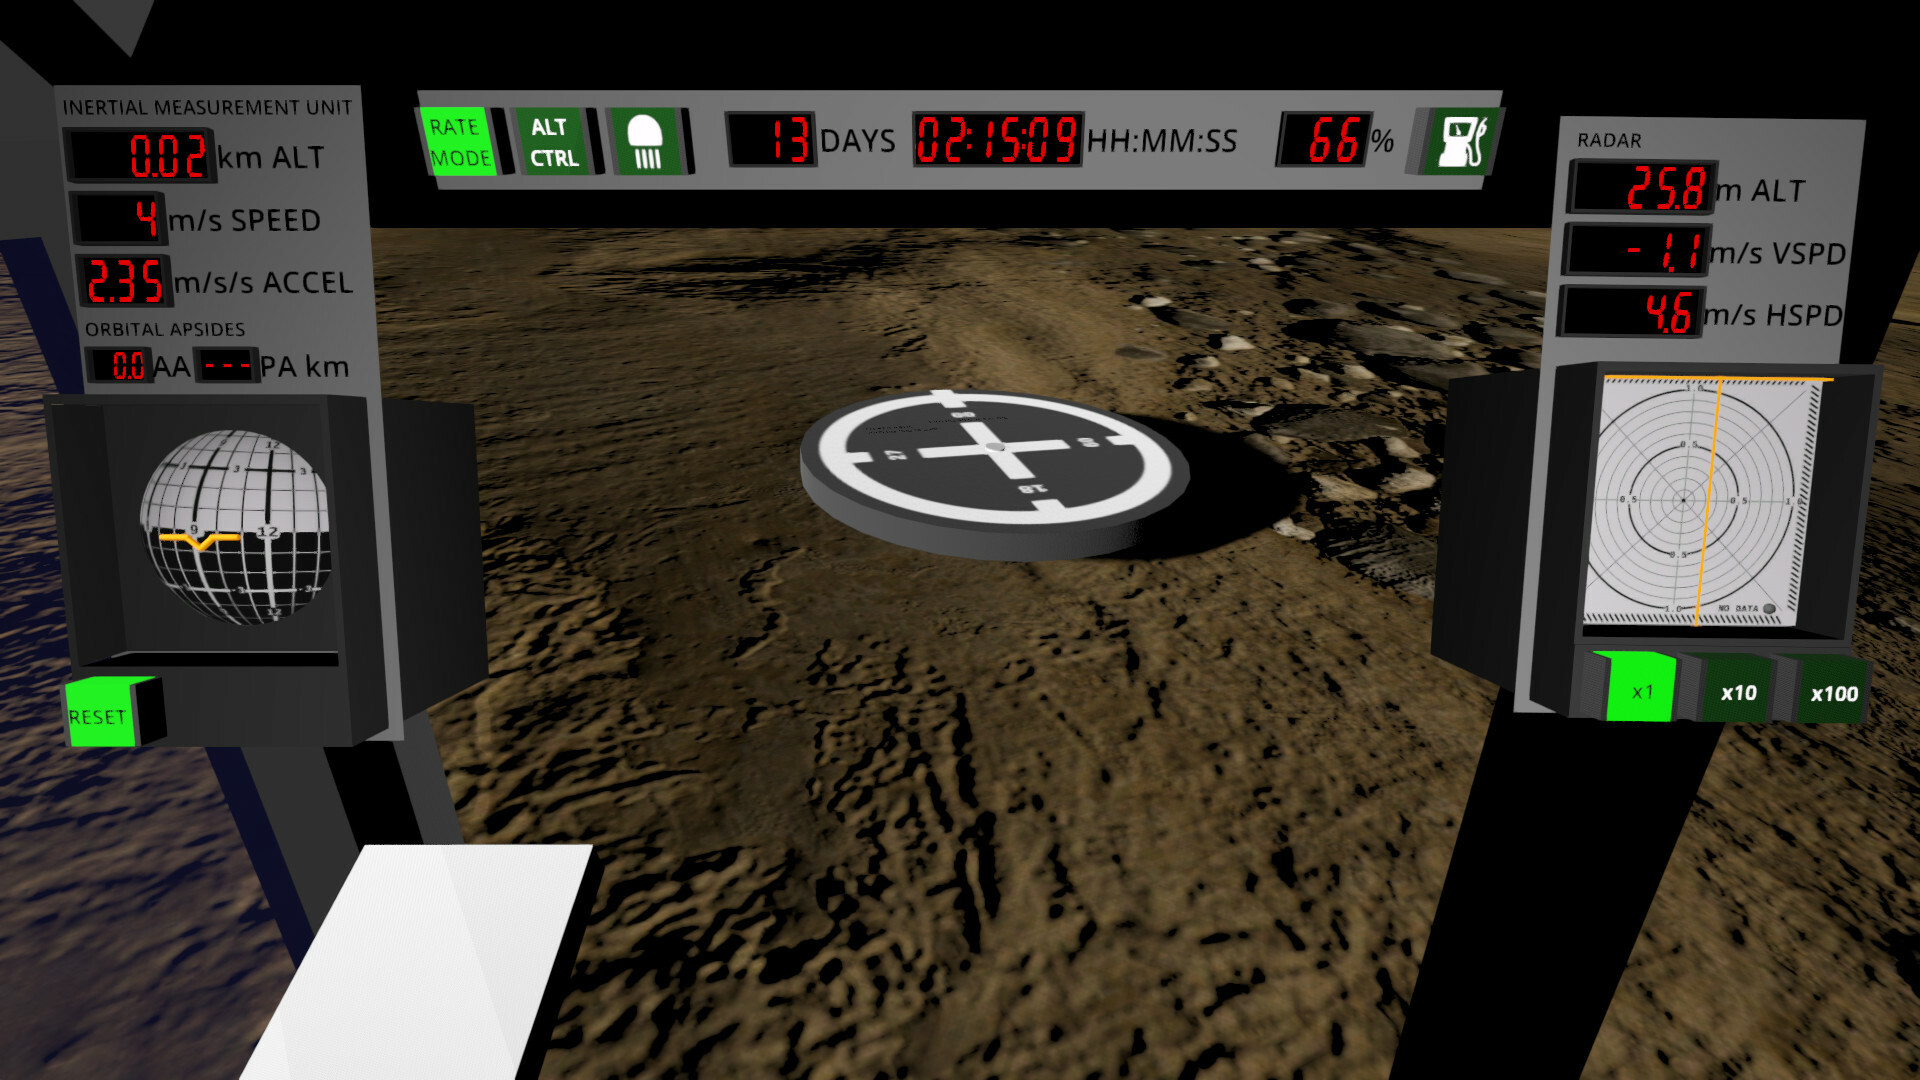
\includegraphics[width=\textwidth]{tungsten-moon}\\
      \href{https://tungstenmoon.com/}{Tungsten Moon}\\
      proprietary, demo available, to be released
    \end{center}
  \end{minipage}
  \begin{minipage}[t]{0.49\textwidth}
    \begin{center}
      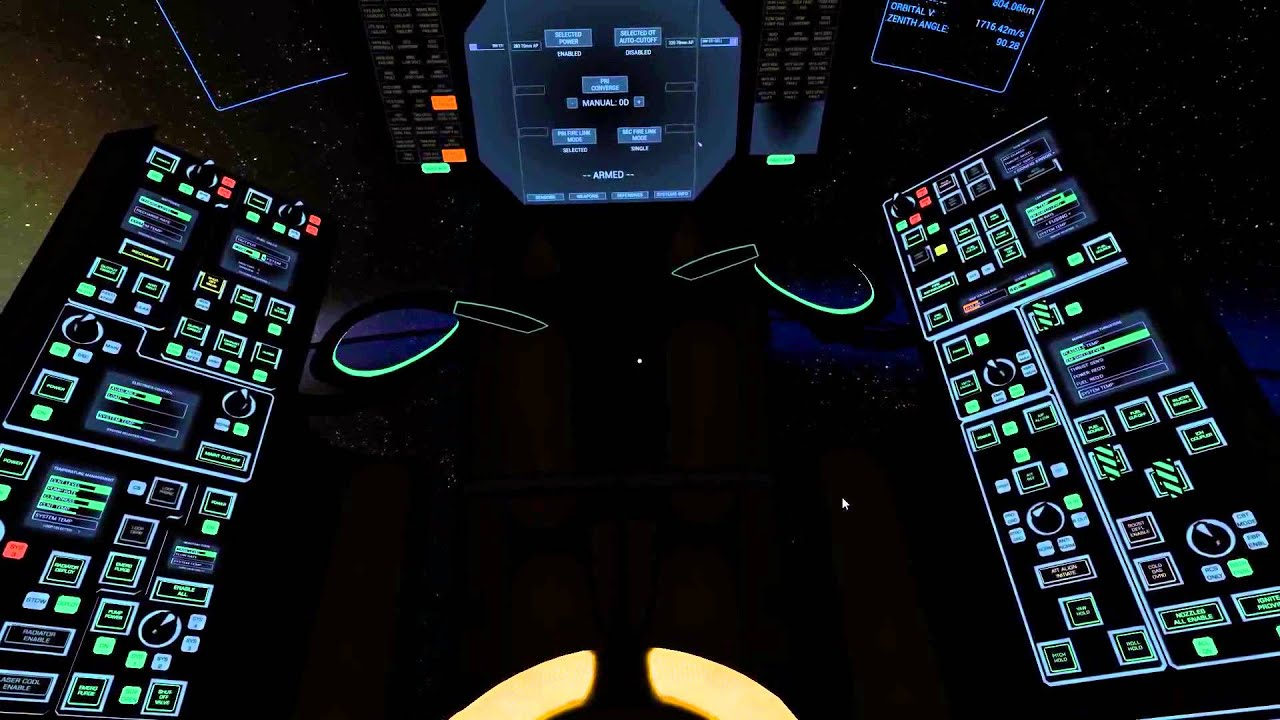
\includegraphics[width=\textwidth]{rogue-system}\\
      \href{https://imagespaceinc.com/rogsys/}{Rogue System}\\
      proprietary, detailed cockpit, released, development on hold
    \end{center}
  \end{minipage}
\end{frame}

\begin{frame}
  \frametitle{Space Flight Simulator Examples}
  \begin{minipage}[t]{0.49\textwidth}
    \begin{center}
      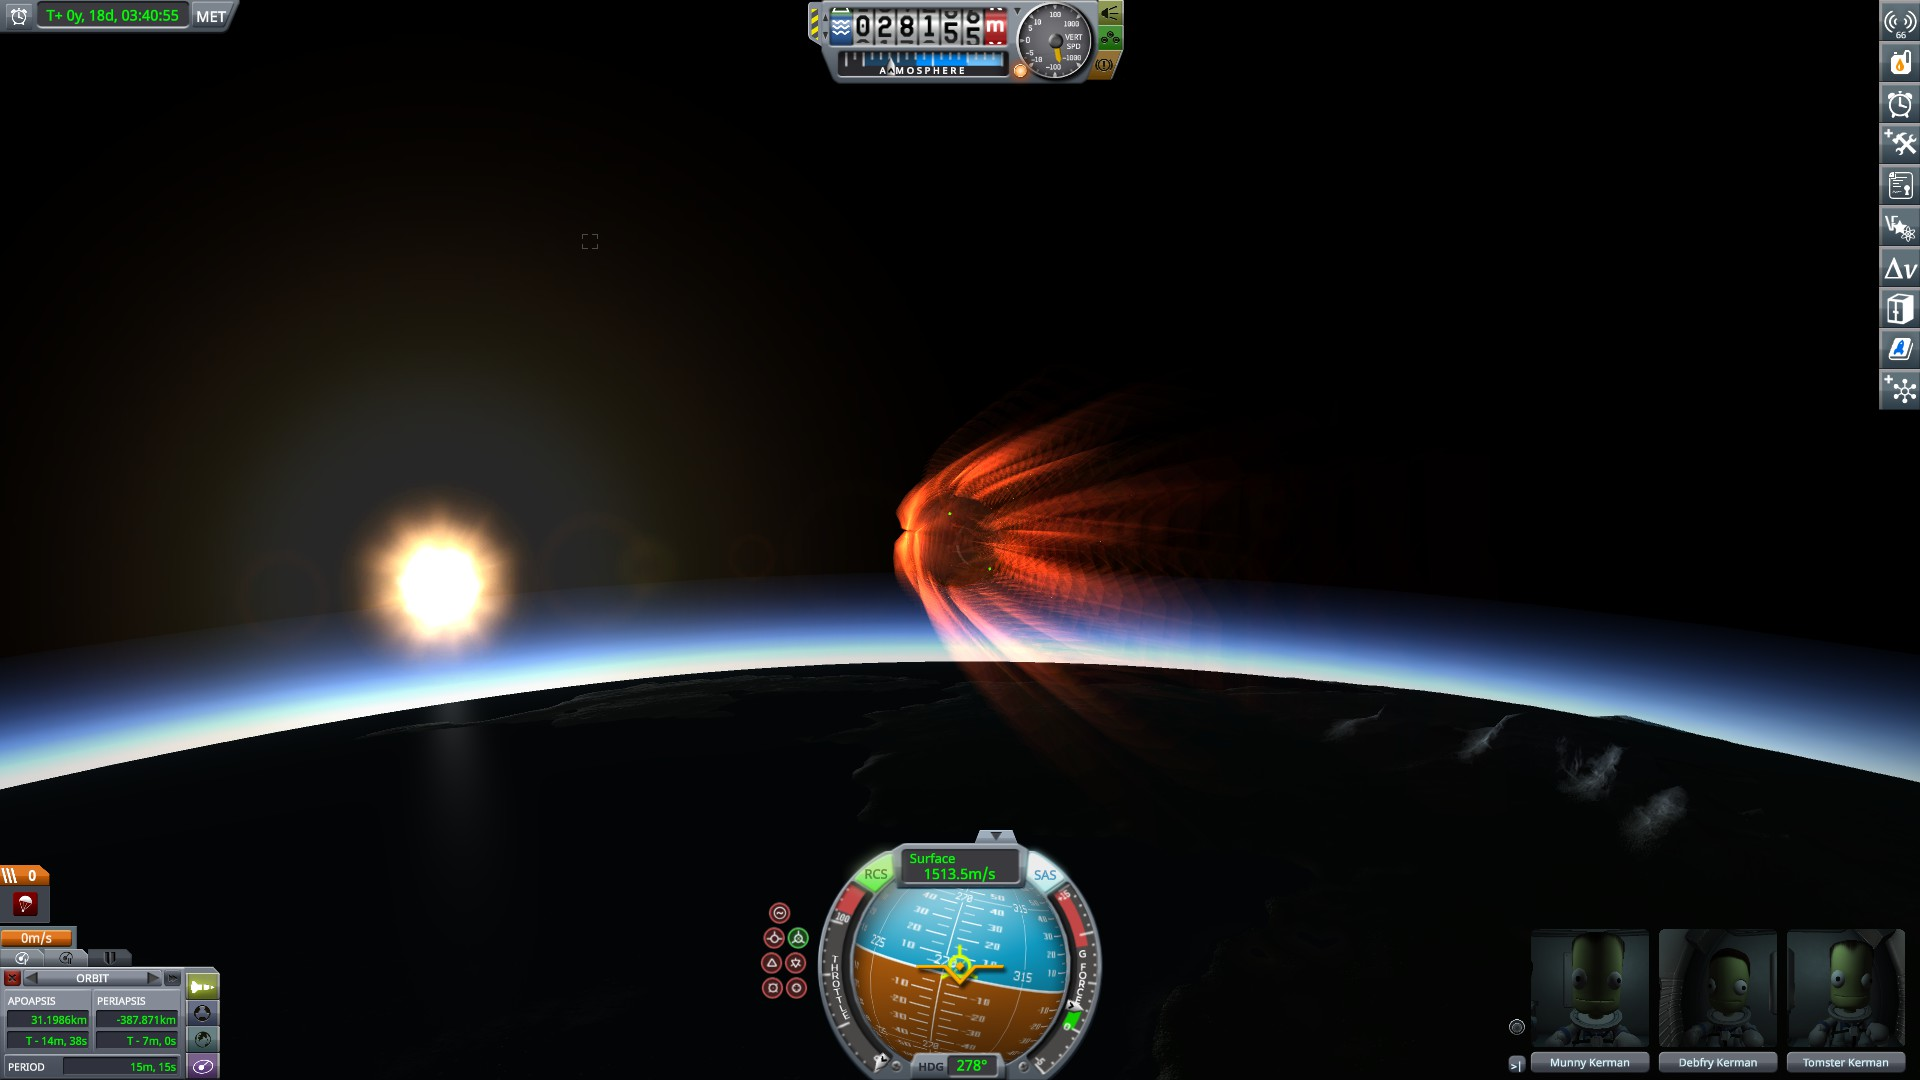
\includegraphics[width=\textwidth]{ksp}\\
      \href{https://www.kerbalspaceprogram.com/}{Kerbal Space Program}\\
      proprietary, realistic, small scale planets, many mods, KSP 2 team disbanded
    \end{center}
  \end{minipage}
  \begin{minipage}[t]{0.49\textwidth}
    \begin{center}
      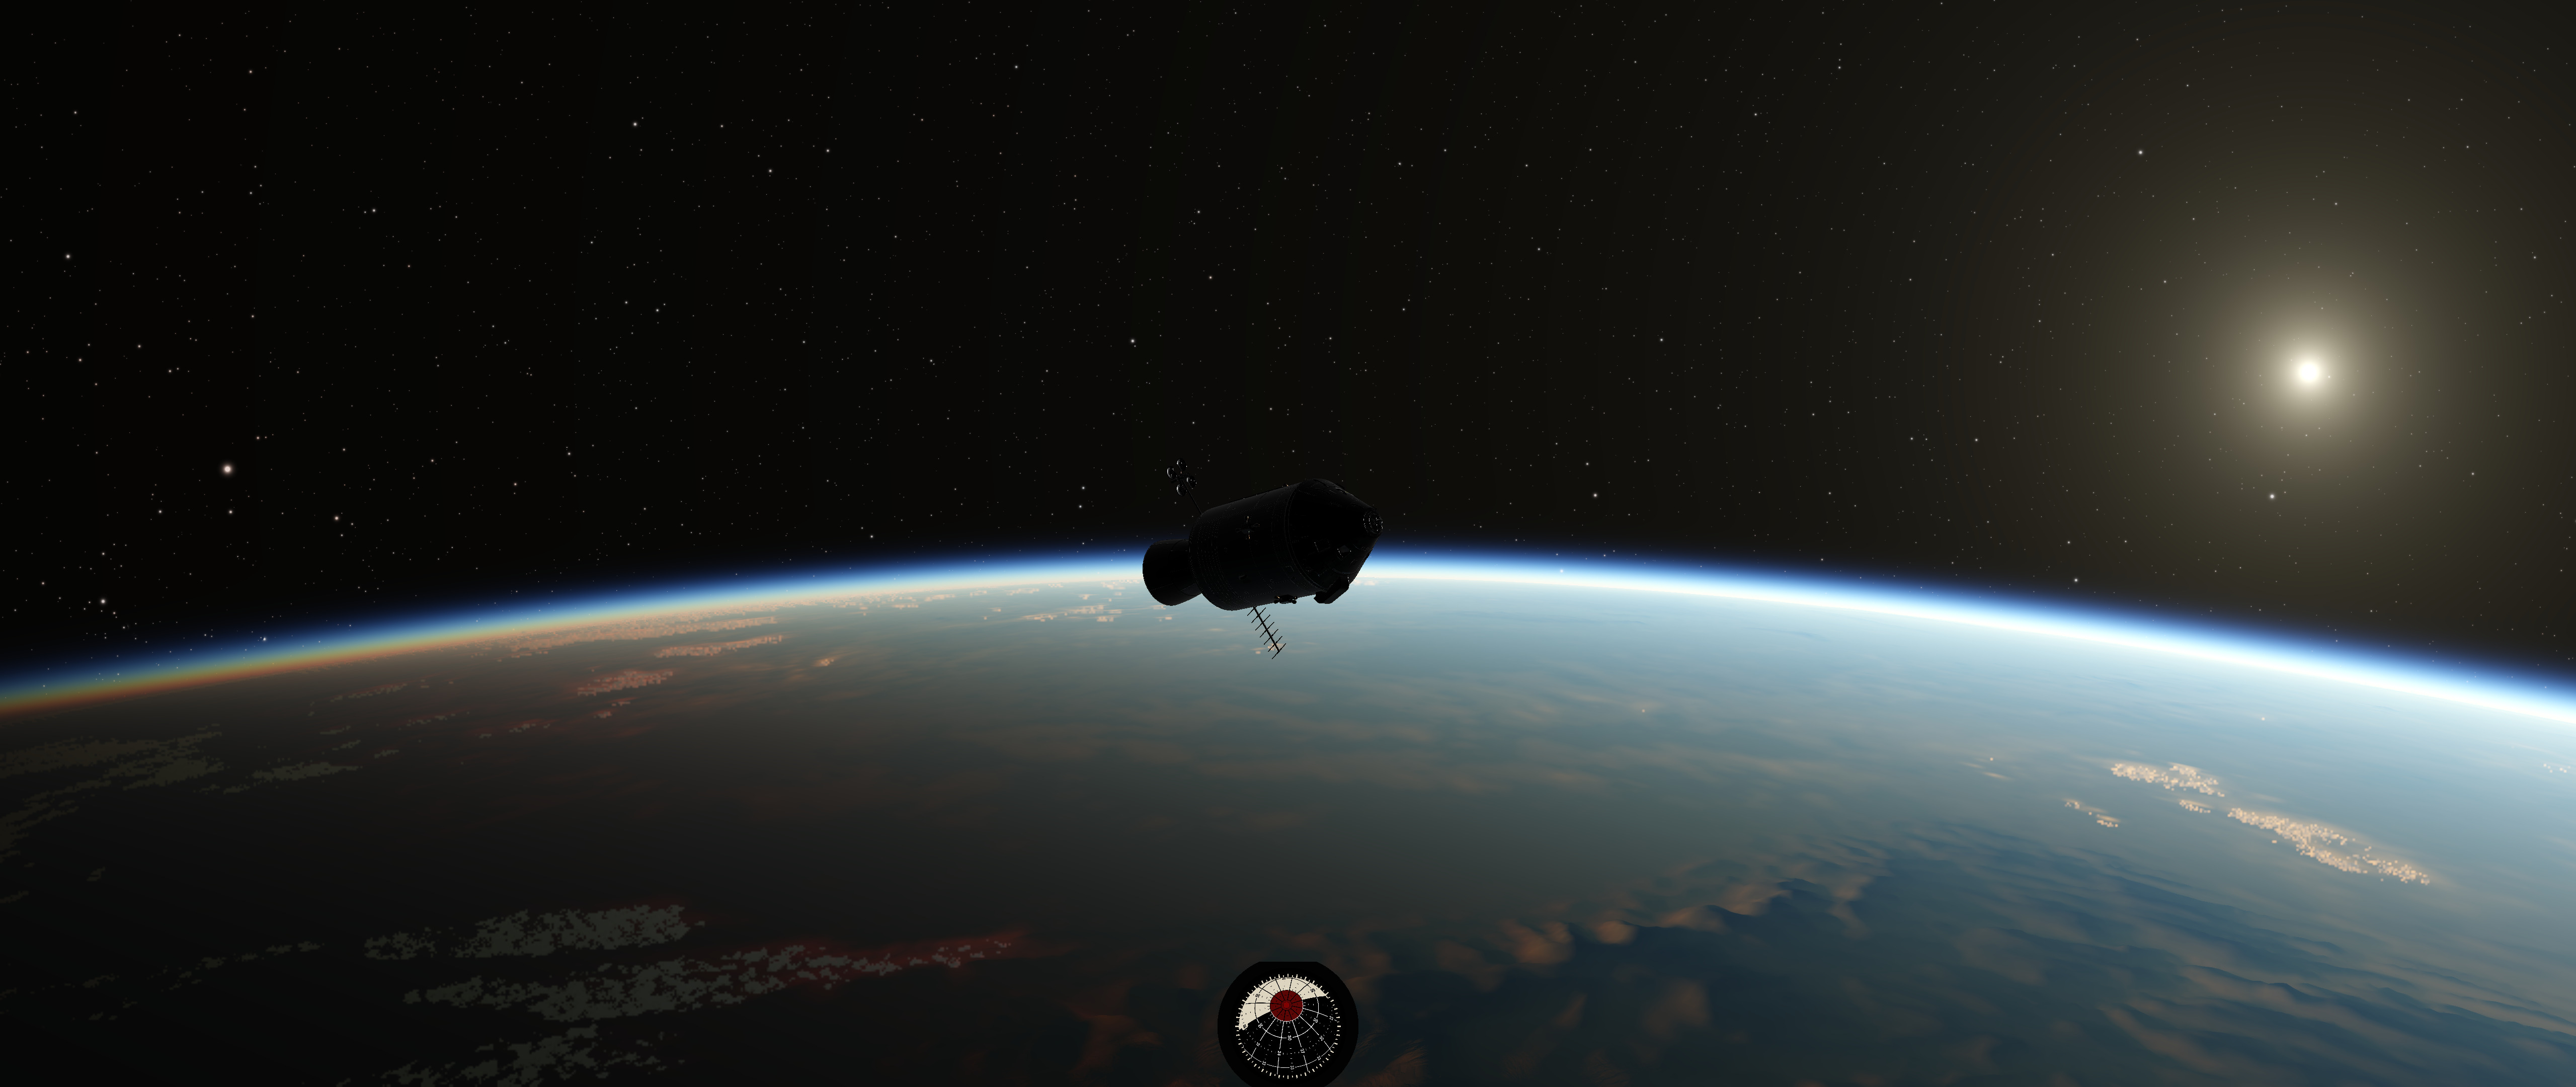
\includegraphics[width=\textwidth]{ksa}\\
      \href{https://rocketwerkz.com/}{Kitten Space Agency}\\
      proprietary, realistic, spiritual successor to KSP 2
    \end{center}
  \end{minipage}
\end{frame}

\begin{frame}
  \pdfbookmark[1]{Motivation}{motivation}
  \frametitle{Motivation}
  \begin{minipage}[t]{0.49\textwidth}
    Develop a space flight simulator
    \begin{itemize}
      \item \textbf{Realistic Physics}
      \item \textbf{Software Libre}
      \item \textbf{High-Level Programming Language}
      \item Realistic Celestial Motions
      \item Cross Platform
    \end{itemize}
  \end{minipage}
  \begin{minipage}[t]{0.49\textwidth}
    Limit scope for now
    \begin{itemize}
      \item One Spacecraft with 3D cockpit
      \item Earth, Sun, and Moon only
      \item Launch pad, runway, space station, moon base
    \end{itemize}
  \end{minipage}
\end{frame}

\begin{frame}
  \pdfbookmark[1]{OpenGL Superbible}{superbible}
  \frametitle{OpenGL Superbible}
  \begin{center}
    
\includegraphics[width=.35\textwidth]{superbible}\\
    \url{https://tinyurl.com/superbible}
  \end{center}
\end{frame}

\begin{frame}[fragile]
  \pdfbookmark[1]{Plain Window}{plainwindow}
  \pdfbookmark[2]{Dependencies}{plainwindowdeps}
  \frametitle{Plain Window {-} Dependencies}
  Using the following \texttt{deps.edn} (replace linux with windows or macos as appropriate):
  \begin{minted}[]{clj}
{:deps {org.clojure/clojure {:mvn/version "1.12.2"}
        generateme/fastmath {:mvn/version "2.4.0"
          :exclusions [com.github.haifengl/smile-mkl org.bytedeco/openblas]}
        org.lwjgl/lwjgl {:mvn/version "3.3.6"}
        org.lwjgl/lwjgl$natives-linux {:mvn/version "3.3.6"}
        org.lwjgl/lwjgl-opengl {:mvn/version "3.3.6"}
        org.lwjgl/lwjgl-opengl$natives-linux {:mvn/version "3.3.6"}
        org.lwjgl/lwjgl-glfw {:mvn/version "3.3.6"}
        org.lwjgl/lwjgl-glfw$natives-linux {:mvn/version "3.3.6"}
        org.lwjgl/lwjgl-stb {:mvn/version "3.3.6"}
        org.lwjgl/lwjgl-stb$natives-linux {:mvn/version "3.3.6"}}
 :paths ["."]}
  \end{minted}
\end{frame}

\begin{frame}[fragile]
  \pdfbookmark[2]{Create}{plainwindowcreate}
  \frametitle{Plain Window {-} Create}
  Initialise GLFW library and create a window with OpenGL context:
  \begin{minted}[]{clj}
(import '[org.lwjgl.glfw GLFW]
        '[org.lwjgl.opengl GL GL11])

(GLFW/glfwInit)

(def window-width 1280)
(def window-height 720)

(GLFW/glfwDefaultWindowHints)
(def window
     (GLFW/glfwCreateWindow window-width window-height "example" 0 0))

(GLFW/glfwShowWindow window)
(GLFW/glfwMakeContextCurrent window)
(GL/createCapabilities)
  \end{minted}
\end{frame}

\begin{frame}[fragile]
  \pdfbookmark[2]{Event Loop}{plainwindowloop}
  \frametitle{Plain Window {-} Event Loop}
  Run event loop as follows:
  \begin{minted}[]{clj}
(while (not (GLFW/glfwWindowShouldClose window))
       (GL11/glClearColor 0.0 1.0 0.0 1.0)
       (GL11/glClear GL11/GL_COLOR_BUFFER_BIT)
       (GLFW/glfwSwapBuffers window)
       (GLFW/glfwPollEvents))
  \end{minted}
\end{frame}

\begin{frame}[fragile]
  \pdfbookmark[2]{Terminate}{plainwindowterminate}
  \frametitle{Plain Window {-} Terminate}
  Terminate the program like this:
  \begin{minted}[]{clj}
(GLFW/glfwDestroyWindow window)
(GLFW/glfwInit)
(GLFW/glfwTerminate)
  \end{minted}
\end{frame}

\begin{frame}
  \pdfbookmark[2]{Result}{plainwindowresult}
  \frametitle{Plain Window {-} Result}
  \begin{center}
    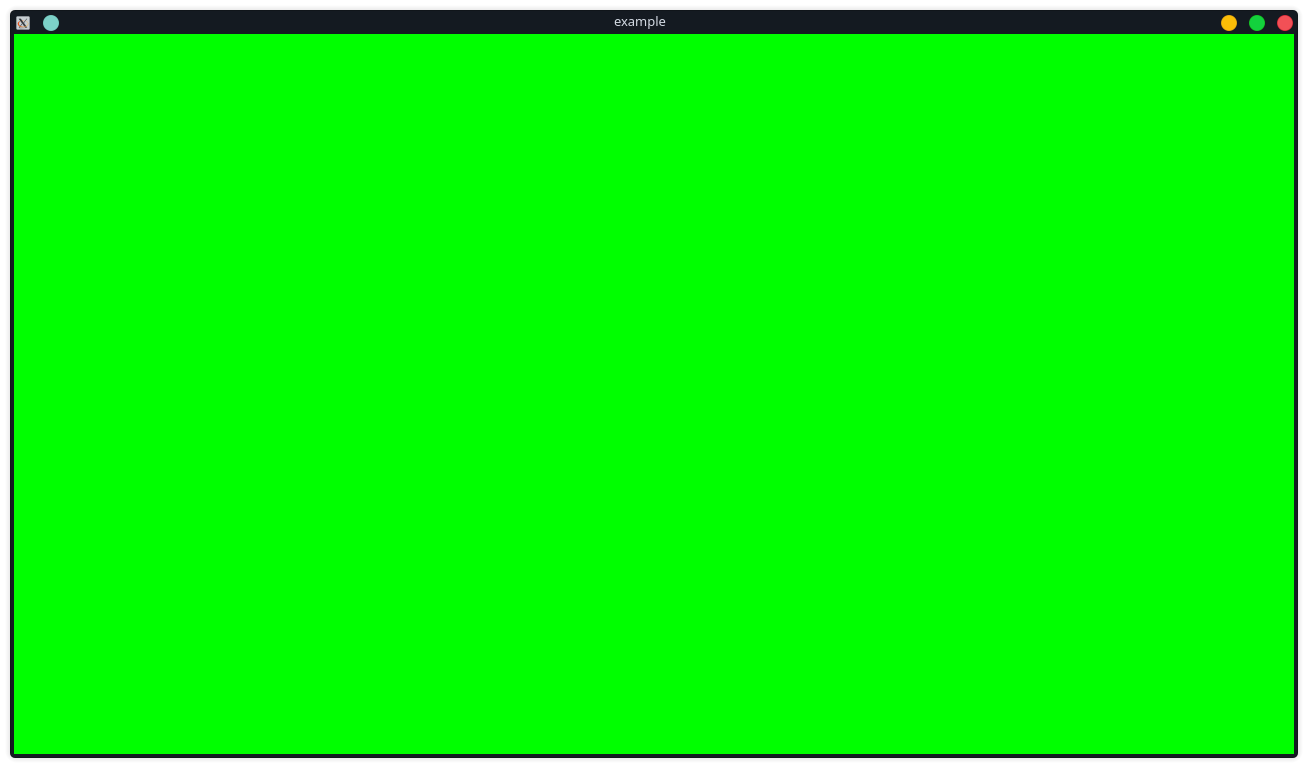
\includegraphics[width=.8\textwidth]{window}
  \end{center}
\end{frame}

\begin{frame}[fragile]
  \pdfbookmark[1]{Single Quad}{quad}
  \pdfbookmark[2]{Import}{quadimport}
  \frametitle{Single Quad {-} Import}
  \begin{minted}[]{clj}
(import '[org.lwjgl.glfw GLFW]
        '[org.lwjgl.opengl GL GL11 GL15 GL20 GL30]
        '[org.lwjgl BufferUtils])
  \end{minted}
\end{frame}

\begin{frame}[fragile]
  \pdfbookmark[2]{Vertex Shader}{quadvertex}
  \frametitle{Single Quad {-} Vertex Shader}
  \begin{minted}[]{clj}
(def vertex-source "
#version 130

in vec3 point;

void main()
{
  gl_Position = vec4(point, 1);
}")
  \end{minted}
\end{frame}

\begin{frame}[fragile]
  \pdfbookmark[2]{Fragment Shader}{quadvertex}
  \frametitle{Single Quad {-} Fragment Shader}
  \begin{minted}[]{clj}
(def fragment-source "
#version 130

uniform vec2 iResolution;
out vec4 fragColor;

void main()
{
  vec2 uv = gl_FragCoord.xy / iResolution.xy;
  fragColor = vec4(uv, 0, 1);
}")
  \end{minted}
\end{frame}

\begin{frame}[fragile]
  \pdfbookmark[2]{Compiling Shaders}{quadcompile}
  \frametitle{Single Quad {-} Compiling Shaders}
  \begin{minted}[]{clj}
(defn make-shader [source shader-type]
  (let [shader (GL20/glCreateShader shader-type)]
    (GL20/glShaderSource shader source)
    (GL20/glCompileShader shader)
    (when (zero? (GL20/glGetShaderi shader GL20/GL_COMPILE_STATUS))
      (throw (Exception. (GL20/glGetShaderInfoLog shader 1024))))
    shader))

(def vertex-shader (make-shader vertex-source GL20/GL_VERTEX_SHADER))
(def fragment-shader (make-shader fragment-source GL20/GL_FRAGMENT_SHADER))
  \end{minted}
\end{frame}

\begin{frame}[fragile]
  \pdfbookmark[2]{Linking Shader Program}{quadcompile}
  \frametitle{Single Quad {-} Linking Shader Program}
  \begin{minted}[]{clj}
(defn make-program [& shaders]
  (let [program (GL20/glCreateProgram)]
    (doseq [shader shaders]
           (GL20/glAttachShader program shader)
           (GL20/glDeleteShader shader))
    (GL20/glLinkProgram program)
    (when (zero? (GL20/glGetProgrami program GL20/GL_LINK_STATUS))
      (throw (Exception. (GL20/glGetProgramInfoLog program 1024))))
    program))

(def program (make-program vertex-shader fragment-shader))
  \end{minted}
\end{frame}

\begin{frame}
  \pdfbookmark[1]{questions}{questions}
  \begin{center}
    \begin{huge}
      Thanks for listening!
    \end{huge}
  \end{center}
\end{frame}

\end{document}
